\documentclass[10pt,a4paper]{article}
\usepackage[utf8]{inputenc}

% Define the page margin
\usepackage[margin=3cm]{geometry}

% Better typography (font rendering)
\usepackage{microtype}

% Math environments and macros
\usepackage{amsmath}
\usepackage{amsfonts}
\usepackage{amssymb}
\usepackage{amsthm}

% Define \includegraphics to include graphics
\usepackage{graphicx}

% Draw graphics from a text description
\usepackage{tikz}

% Syntax highlighting
\usepackage{minted}

% Set global minted options
\setminted{linenos, autogobble, frame=lines, framesep=2mm}

% Import the comment environment for orgtbl-mode
\usepackage{comment}

% Do not indent paragraphs
\usepackage{parskip}

\title{Randomized Algorithms, Sheet 5}
\author{Marten Lienen (03670270)}

\begin{document}

\maketitle

\section*{Exercise 5.1}

\begin{proof}
  As an input pick a permutation of the numbers $1, \dots, n$ uniformly at random.

  We can now model any run of a deterministic comparison-based algorithm as a decision tree as hinted on the exercise sheet.
  In such a decision tree the leaves are the resulting sorted sequences.
  Since there are $n!$ different possible permutations of $n$ numbers, any decision tree of a comparison-based deterministic algorithm has to have at least $n!$ leaves.
  If it had less, there would be at least two sortings that the algorithm could not distinguish.
  The expected number of comparisons is then the expected depth of this tree.
  At this point we can, however, find a lower bound for this.
  A complete binary tree with $n!$ leaves has a depth of $\log(n!)$.
  This means that you need $\log(n!)$ decisions to distinguish between the $n!$ different possible sortings.
  As a consequence no decision tree can have a leaf at a depth less then $\log(n!)$ because it would not have made sufficiently many comparisons to distinguish between at least two sortings.
  So no comparison-based deterministic sorting algorithm can do better than a decision tree with every leaf at a depth of $\log(n!)$.
  Now we have shown that $\log(n!)$ is a lower bound for the expected run time of any such sorting algorithm, in particular for the best one, and we can rewrite it as
  \begin{align*}
    \log(n!) & = \log\left( \prod_{i = 1}^{n} i \right)\\
             & = \sum_{i = 1}^{n} \log(i)\\
             & \ge \sum_{i = \lceil \frac{n}{2} \rceil}^{n} \log\left( \lceil \frac{n}{2} \rceil \right)\\
             & = \left( n - \lceil \frac{n}{2} \rceil + 1 \right) \cdot \log\left( \lceil \frac{n}{2} \rceil \right)\\
             & \ge \frac{n}{2} \cdot \log\left( \frac{n}{2} \right) = \frac{1}{2}n \log(n) - \frac{n}{2} \cdot \log(2) \in \mathcal{O}(n\log(n))
  \end{align*}
  This proves that no deterministic algorithm can do less comparisons than $\mathcal{O}(n\log(n))$ and by Yao's minimax principle neither can the best randomized algorithm.
\end{proof}

\section*{Exercise 5.2}

\begin{proof}
  We begin by defining a distribution over bit vectors of length $n$.
  With probability $\frac{1}{2}$ we pick a vector of $n$ zeros.
  With the counter probability of $\frac{1}{2}$ we pick a bit vector that has exactly two consecutive ones, namely at position $y$ and $y + 1$ where we pick $y$ uniformly from $\{ 1, \dots, n - 1 \}$.

  The main observation is that any algorithm can check all possible positions of the pair of ones in $\lceil \frac{n - 1}{2} \rceil$ inspections by checking every second slot starting at the second position so that there are no two consecutive unchecked positions.
  If it inspected less, there would be at least two consecutive uninspected positions where two ones could ``hide'' by the pigeon hole principle.
  So any algorithm has to perform at least $\lceil \frac{n - 1}{2} \rceil$ inspections in the case of a bit string of all zeros.

  In the case of a string with a pair of ones, the algorithm still has to check potentially all these positions until it finds consecutive ones.
  Since the position of the pair of ones is uniformly distributed over the positions $1, \dots, n - 1$, the number of inspections until the algorithm finds the pair is also uniformly distributed over $1, \dots, \lceil \frac{n - 1}{2} \rceil$.
  Therefore the expected number of inspections is
  \begin{align*}
    \frac{1}{2} \cdot \lceil \frac{n - 1}{2} \rceil + \frac{1}{2} \cdot \sum_{k = 1}^{\lceil \frac{n - 1}{2} \rceil} k \cdot \frac{1}{\lceil \frac{n - 1}{2} \rceil} = & \frac{1}{2} \cdot \lceil \frac{n - 1}{2} \rceil + \frac{1}{2} \cdot \frac{1}{\lceil \frac{n - 1}{2} \rceil} \cdot \sum_{k = 1}^{\lceil \frac{n - 1}{2} \rceil} k\\
                                                                                                                                                                       & = \frac{1}{2} \cdot \lceil \frac{n - 1}{2} \rceil + \frac{1}{2} \cdot \frac{1}{\lceil \frac{n - 1}{2} \rceil} \cdot \frac{\lceil \frac{n - 1}{2} \rceil (\lceil \frac{n - 1}{2} \rceil + 1)}{2}\\
                                                                                                                                                                       & = \frac{1}{2} \cdot \left( \lceil \frac{n - 1}{2} \rceil + \frac{\lceil \frac{n - 1}{2} \rceil + 1}{2} \right)\\
                                                                                                                                                                       & \ge \frac{1}{2} \cdot \left(  \frac{n - 1}{2} - 1 + \frac{\frac{n - 1}{2} - 1 + 1}{2} \right)\\
                                                                                                                                                                       & = \frac{1}{2} \cdot \left(  \frac{n - 3}{2} + \frac{n - 1}{4} \right) = \frac{1}{2} \cdot \frac{3n - 7}{4} \in \mathcal{O}(n)
  \end{align*}
  Yao's minimax principle asserts that this is a lower bound for the number of inspections of the best randomized algorithm.
  In other words the expected number of bits inspected by the best and thus any randomized algorithm is in $\Theta(n)$.
\end{proof}

\section*{Exercise 5.3}

\subsection*{Part a}

\begin{proof}
  Define a random variable $X \in \{ 1, \dots, n \}$ as the number of probes needed and another random variable $Y \in \{ 1, \dots, n \}$ as the position of the bill.
  Then we can give the probability of a specific value for $X$ as
  \begin{equation*}
    P[X = k] = P[Y = k \mid x = H] + P[Y = n + 1 - k \mid x = T]
  \end{equation*}
  Therefore the expected value of $X$ is
  \begin{align*}
    E[X] & = \sum_{k = 1}^{n} k \cdot P[X = k]\\
         & = \sum_{k = 1}^{n} k \cdot \left( P[Y = k \mid x = H] + P[Y = n + 1 - k \mid x = T] \right)\\
         & = \sum_{k = 1}^{n} k \cdot \left( \frac{1}{2} \cdot \left( \frac{1}{n} + \frac{1}{n} \right) \right)\\
         & = \frac{1}{n} \cdot \sum_{k = 1}^{n} k = \frac{1}{n} \cdot \frac{n(n + 1)}{2} = \frac{n + 1}{2}
  \end{align*}
\end{proof}

\subsection*{Part b}

\begin{proof}
  Using Yao's minimax principle we can prove this lower bound by computing the minimum expected run time of any deterministic algorithm for a given input distribution.
  Let the position $y$ of the bill be uniformly distributed over $1, \dots, n$.

  The important observation is that every deterministic algorithm will perform probes until it finds the bill and the order of these probes before it is successful will be the same regardless of the bill position $y$.
  The reason is that two runs for e.g. $y = y_{1}$ and $y = y_{2}$ look exactly the same for the first $\min(y_{1}, y_{2}) - 1$ iterations.
  Consequently the algorithm has to take the same decisions at each step.

  After this insight we know that every deterministic algorithm has a fixed order of probing the boxes.
  Without loss of generality we can assume this order to be $1, \dots, n$ since we can rename the boxes otherwise.
  Then we are basically in the scenario of part $1$ again and the expected number of probes of any deterministic algorithm is
  \begin{equation*}
    \sum_{k = 1}^{n} k \cdot P[y = k] = \sum_{k = 1}^{n} k \cdot \frac{1}{n} = \frac{1}{n} \cdot \sum_{k = 1}^{n} k = \frac{1}{n} \cdot \frac{n(n + 1)}{2} = \frac{n + 1}{2}
  \end{equation*}
  which is thus also a lower bound for the number of probes for any and in particular the best randomized algorithm.
\end{proof}

\section*{Exercise 5.4}

The following equivalence can be easily verified with a truth table.

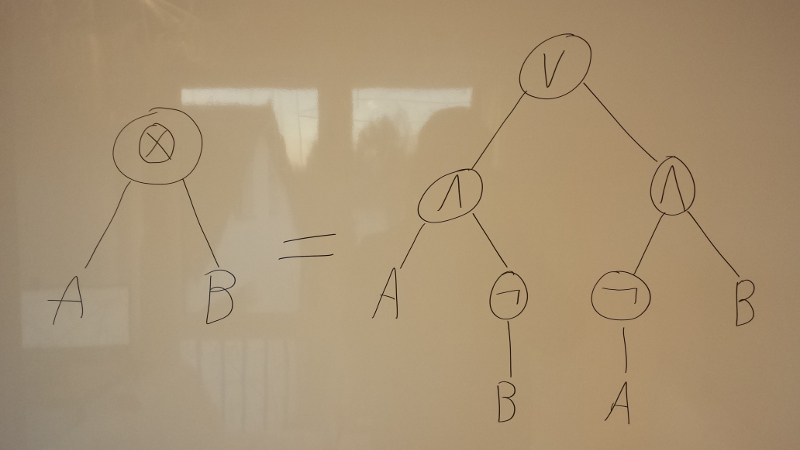
\includegraphics[width=\textwidth]{sheet-5/exercise-4-1}

A boolean circuit is an acyclic directed graph without any restriction on the out-degrees.
Hence we can reuse expressions in the boolean circuit by giving vertices multiple out-edges.

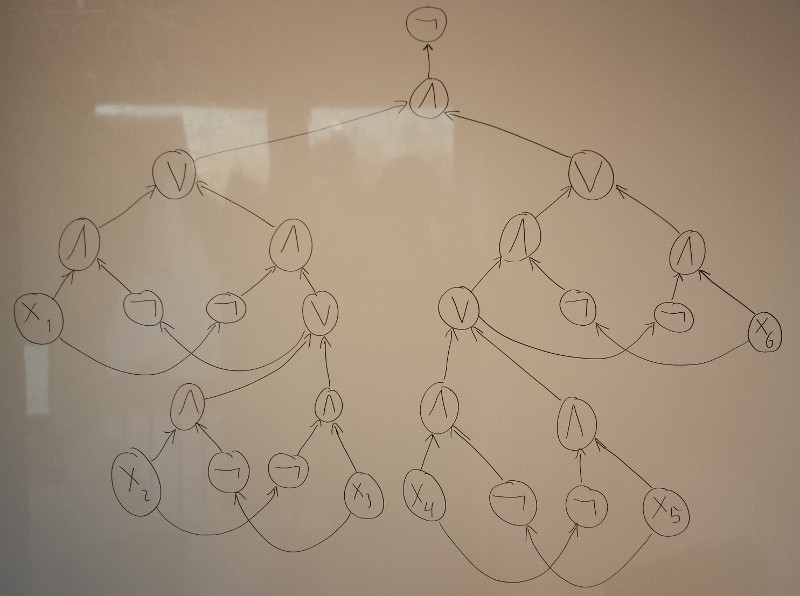
\includegraphics[width=\textwidth]{sheet-5/exercise-4-2}

\end{document}
